\section{Introduction}

Imagine you just moved to the United States and are visiting Target for the first time. Perhaps since you just moved in, your first goal is to furnish your apartment. You look around at the entrance, and navigate your way to the furniture section perhaps while taking a few false turns on the way, buy the stuff you need, pay and leave. The next time you visit for, for example, groceries and produce. You visit again for sporting goods and then again for gifts for your friends. An year later, all such subset of visits through the Target store makes you an expert in knowing the specific route to the section you need to visit. What algorithmic mechanisms allow us to build such expertise to create connections in an explored environment even when during no single visit, you explored all possible connections between regions of the store?

We are able to build up a map of the environment without being exposed to the full extent of it in a single iteration simply based on local exposures to it. Such building is often implicit -- you just know that in order to go to the furniture area, you need to pass through the gifts even when you did not explicitly explore this connection before. In this chapter I explore some algorithmic mechanisms that may lead to our ability to acquire large-scale structural knowledge of the environment based on local exposures. 

The effect of local exposure in acquiring structural knowledge of the environment have been explored in several areas of cognitive psychology through artificial grammar and language learning \cite{knowlton1992intact, romberg2010statistical, aslin2012statistical, dehaene2015neural}, visual statistical learning \cite{fiser2002statistical, turk2008multidimensional, brady2008statistical}, or motor sequence learning \cite{baldwin2008segmenting, nissen1987attentional, cleeremans1991learning, kahn2018network}. In recent work, (implicit) acquisition of higher order knowledge of the environment from lower order exposure is studied through structured graph based transitions between stimuli \cite{schapiro2013neural, karuza2017process, kahn2018network, lynn2020humans, lynn2020human, karuza2022value}. For example \cite{schapiro2013neural} show that when asked to respond to arbitrary stimuli arranged in a temporally graph-modular structure, participants often parse the edges that connect two modules as `natural breaks' even when their local exposure does not distinguish between the cross-module and within-module edges. 

More commonly, global-scale structure acquisition has been attributed to response time measurements. Earlier work in serial reaction time tasks \cite{nissen1987attentional, cleeremans1991learning} shows that breaking an implicitly learned motor sequence leads to slower reaction times. The slowed reaction times when crossing the between-module edges have also been shown in recent work on statistical learning in modular graph structures \cite{kahn2018network, lynn2020humans, karuza2017process, karuza2022value, karuza2019human, lynn2020human}. 

This slowdown across module edges appears to be mediated by the nature of the walk experienced across the community structure where random and Eulerian walk (a walk where each edge of the graph is visited exactly once before repeats) experiences continue to show this slowdown whereas a Hamiltonian walk (a walk were each node of the graph is visited exactly once before repeats) experience does not \cite{karuza2017process}. Thus it appears that the kind of experience through the graph alters the knowledge of underlying statistical patterns. Similarly, the topographical structure of a graph in motor skill learning tasks also appears to alter structural knowledge \cite{lynn2020abstract, lynn2020human, lynn2020humans} where modular graphs like in Figure \ref{fig:modular_graph} produce the largest dip in reaction times when responding to boundary items.

\begin{figure}
	\centering
	\caption{Modular graph structure used in \cite{schapiro2013neural}. Locally, each node is connected to four nodes with each edge equally probable. However, globally, the graph structure consists of three sub-modules interconnected through `boundary nodes'}
	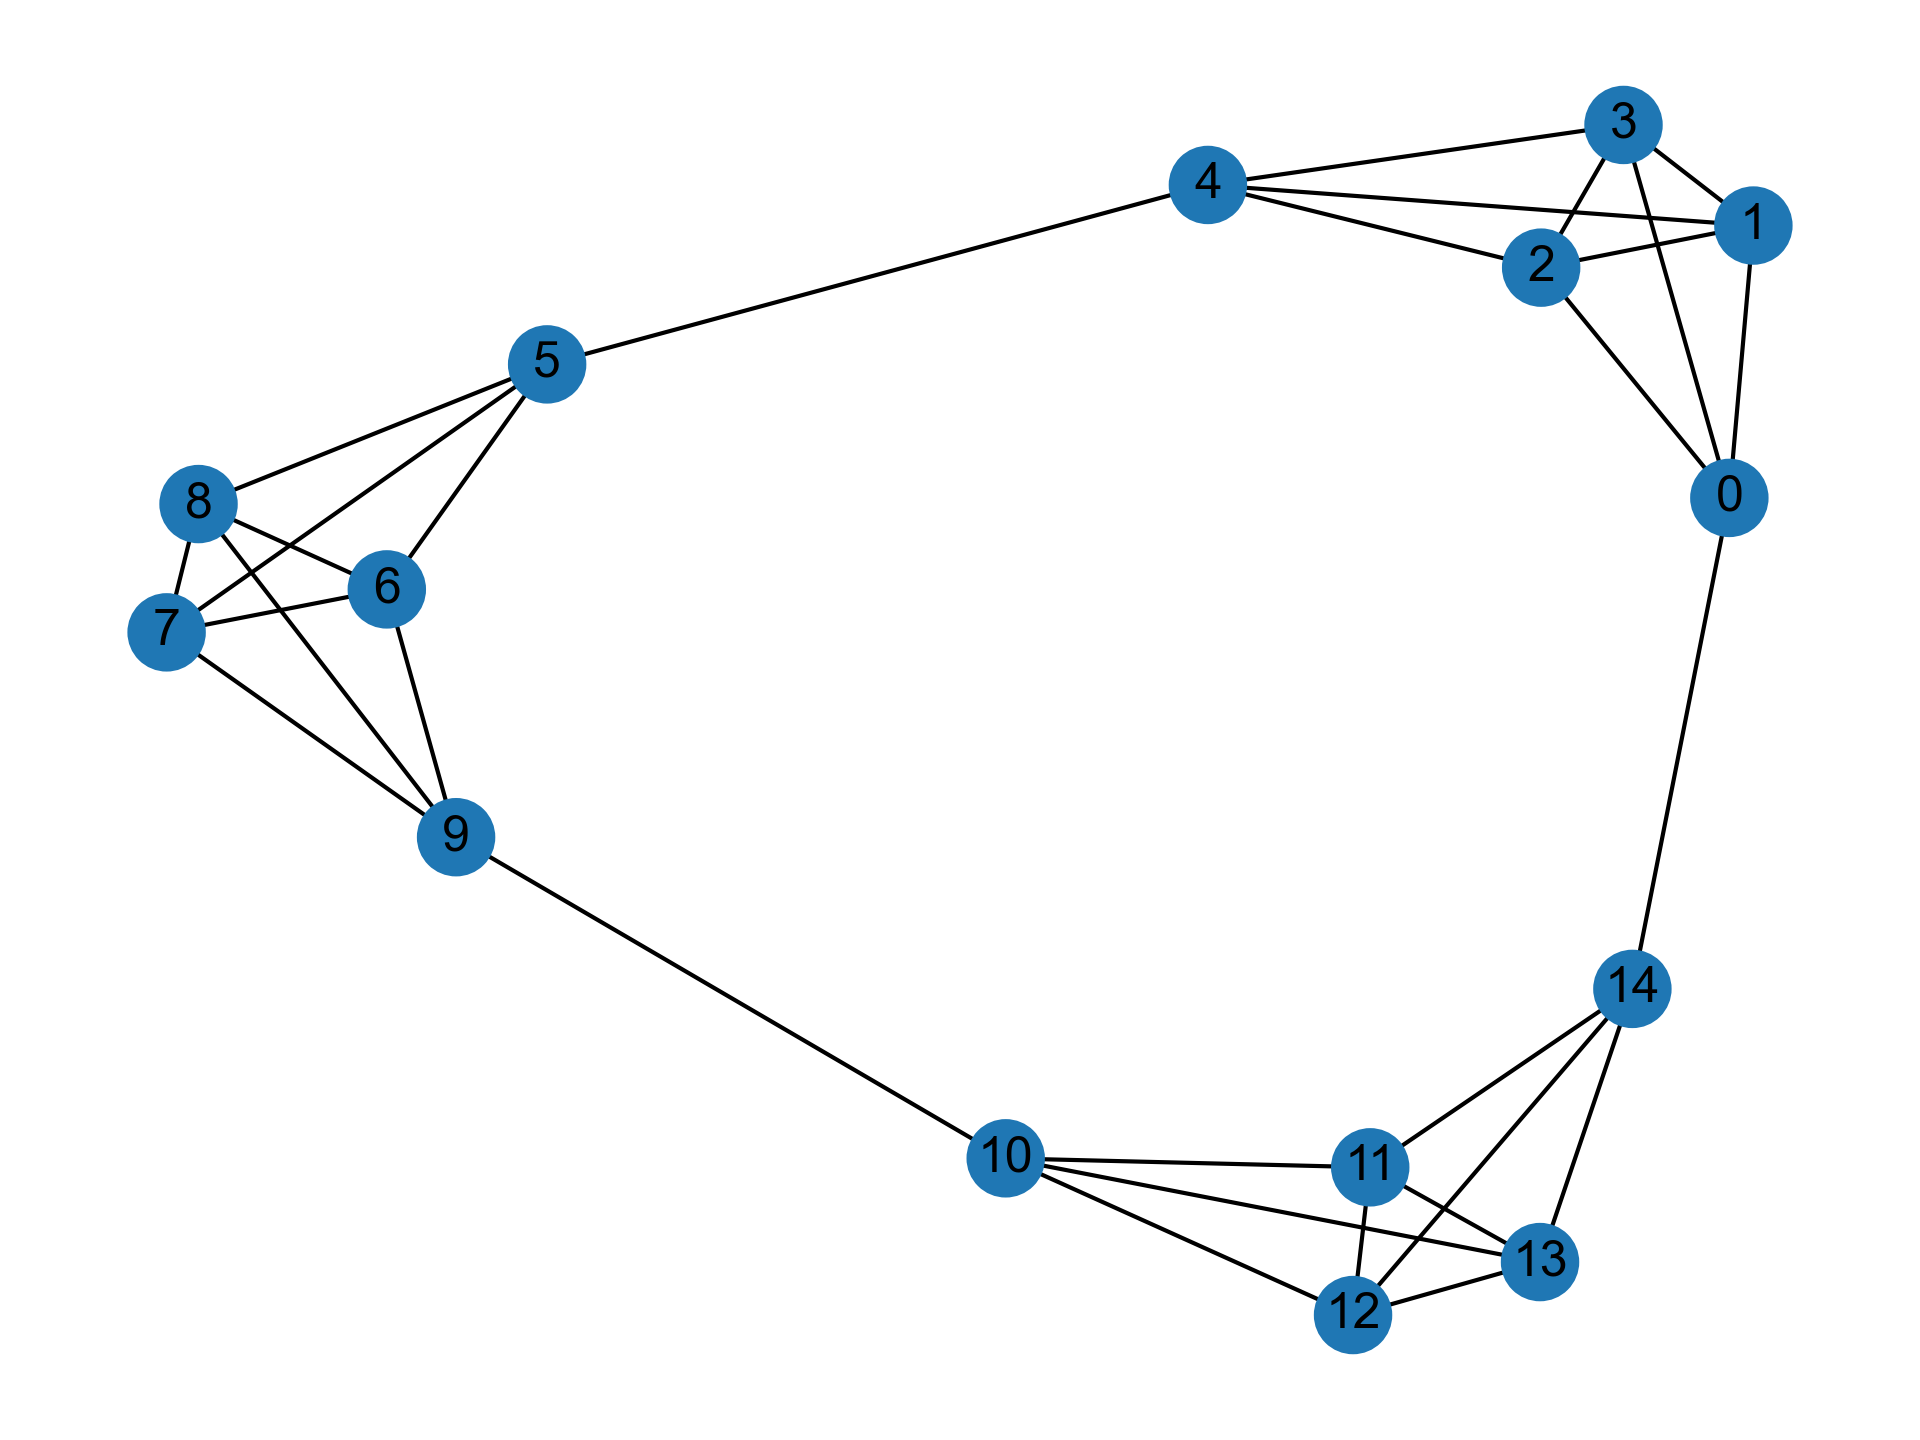
\includegraphics[width = \textwidth]{chapter_notebooks/chapter_2/figures/modular_graph.png}
	\label{fig:modular_graph}
\end{figure}

Why do we slow down at boundary nodes that lead to the adjacent module even when the local probability of that particular transition is the same as any other transitions? Understanding this particular property of human behavior may provide deeper insights into what leads to global-scale structure acquisition; after all the only difference between the boundary node and other non-boundary nodes is in context of the global structure of the graph. Event boundary literature (where boundaries are typically operationalized through explicit changes in context) suggests that boundaries alter the predictability of future events and this predictability leads to event segmentation \cite{zacks2007event, clewett2019transcending}. Thus, in implicitly operationalized boundaries such as in serial reaction time tasks, the slowdown at the boundary node may imply a similarly increased uncertainty at boundary nodes leading to slowed responses. Prior work aimed at understanding human representation of graph structures indeed points to an the `cross-entropy' between a learner's estimate of the transition probability and the true transition probability of the environment \cite{lynn2020abstract, lynn2020humans, lynn2020human}. 

%In addition to being uncertain about the immediate next stimulus, participants are also uncertain about switching to a neighboring cluster or staying within the same cluster.

In particular, \cite{lynn2020human} show that algorithms of contextual representations such as the Successor Representation (SR) model in Reinforcement Learning \cite{dayan1993improving, momennejad2017successor, gershman2018successor} or the associative learning based Temporal Context Model (TCM) can naturally lead to an increased cross-entropy for cross cluster transitions relative to within cluster transitions in modular graphs. In this work, by using the framework of cross-entropy to estimate reaction times in a modular graph we aim to 1) Experimentally test the predictions of these two models when exposure through the modular graph structure of is partial and 2) Provide evidence in favor of one of the two models of representation. 

\subsection{Representations of Temporal Context}

\subsubsection{Successor Representation}\label{successor-representation}

The Successor Representation (SR) model of reinforcement learning has been used as a model to understand the generalization of reinforcement learning behavior in large action spaces \cite{dayan1993improving}. In recent work, the SR model has also been shown to be a reliable model for explaining human decision-making behavior in multi-step environments. The model accurately predicted that humans are worse at adapting to changes in the transition probability of a learned environment than to changes in the end-point rewards \cite{momennejad2017successor}. There has been further evidence of SR being represented in the Hippocampal cells which represent space \cite{gershman2018successor, stachenfeld2017hippocampus}.

Briefly, the SR model represents each state in the actionable space as a predictive representation matrix. For an environment of $N$ discrete states, the SR matrix $M$ of size $(N X N)$ maintains expected future visits to a given state from each state. Specifically, element $M_{i,j}$ of the matrix represents the expected future visits to state $j$ from state $i$. This transition matrix is learned over time based on the temporal difference error learning rule. For example, consider at a given point in time, $t$, an agent maintaining the SR matrix is in state $i$. The agent now moves to state $j$ out of the possible $N$ states. The $i^{th}$ row of the SR matrix is updated as follows:

\begin{equation}
	M_{i,j} \leftarrow \hat{M}_{i,j} + \alpha[\delta(s_{t+1},j) + \gamma*\hat{M}_{s_{t+1},j} - \hat{M}_{s_t,j}]
\end{equation}

where $\delta(., .)$ equates to 1 if both arguments are equal otherwise it equates to 0. Thus, the matrix increases the probability of visiting a state $j$ from state $i$ if state $j$ is visited in the current experience and it decreases the probability of visiting all other states from state $i$. Parameter $\alpha$ is a learning rate parameter that determines how much of the previous estimate of visiting state $j$ from $i$ is factored into the current update. Parameter $\gamma$ is a future discount parameter that dictates how much in the future the agent sees -- specifically, a higher value of $\gamma$ indicates future visitations to state $j$ are weighed high in the current update.

\subsection{Temporal Context Model}
The Temporal Context Model (TCM) was devised to explain the primacy and recency effects in human recall and recognition memory \cite{howard2005temporal}. The TCM model assumes that the items maintain a temporal context as they get encoded thus allowing items presented close to the previous items to share such temporal context. Briefly, the TCM can be formalized as \cite{gershman2012successor}:

\begin{equation}
	\begin{aligned}
		t_n = \rho * t_{n-1} + f_n \\ 
		\hat{M}_{i, j} \leftarrow \hat{M}_{i, j} + \alpha f_{n+1} t_{n, i}			
	\end{aligned}
\end{equation}

where $t_n$ is said to be a `context' vector for item $n$. The context drift parameter $\rho$ determines the proportion of the previous elements's context that gets incorporated in the current context. $f_n$ is a one-hot encoded vector for item $n$. The learning rate parameter $\alpha$ determines what proportion of the currently experienced state binds with the existing context. 

The key difference between the two models of temporal context is two fold: (1) SR Relies on error-based learning whereas TCM relies on hebbian, assosciative learning and (2) Through the future discount parameter $\gamma$, SR also learns the predictability observing states in the near future based on the locally experienced transitions \cite{gershman2012successor}.

\subsection{Model Simulations}
The models described above can be used to simulate expected behavior as a function of a range of exposure. Figure \ref{fig:model_simulations} shows the context matrix representation after the models have been simulated for a random walk through the graph structure in \ref{fig:modular_graph} as a result of a random walk, a Hamiltonian walk and an Eulerian walk after 1000 trials. Previous work has shown that participants acquire the global structure of the graph for both the random and Eulerian walk but \textit{not} when exposed to the temporal graph via a Hamiltonian walk. 

To model the observed differences in reaction times and link them to the apparent differences shown in Figure \ref{fig:model_simulations}, we apply principles of information theory. Specifically, we assume that response time for each stimulus is a function of the uncertainty in its surrounding context. Measures of information entropy have previously been used to explain RT differences in various conditions \cite{lynn2020abstract, lynn2020human,lynn2020humans}. 


%The SR model, while underlies the reinforcement learning principle does not rely on the availability of explicit rewards at the end to build a predictive representation for each step. For this dissertation, I will similarly assume that predictive representations are learned from experience through the environment without the need for an explicit goal state.



